\documentclass{article}
\usepackage{palatino}
\usepackage{graphicx}
\usepackage{listings}
\usepackage{url}
\begin{document}

\lstset{ 
  language=C++,
  belowcaptionskip=1\baselineskip,
  xleftmargin=\parindent,
  basicstyle=\footnotesize\ttfamily
 }

\title{Senior Project: GPU Computing}
\author{John Kloosterman \\
  \texttt{john.kloosterman@gmail.com}}
\date{May 2013}
\maketitle


% The final report should be a formal, written paper discussing the nature of the project, the system you built, and the implications for the future. The general sections to include in your final report are as follows:
% Project vision and overview
% Background, including research review
% System design, implementation and testing
% Results and discussion
% Conclusions
% Future work
% Acknowledgements
% References
% Appendixes (if appropriate)
%%%%%%%%%%%%%%%%%%%%%%
\section{Introduction}

Graphics Processing Units (GPUs) are data-parallel processors. Although designed for interactive 3D graphics, they can be used for general-purpose computational tasks, which is called General Purpose GPU (GPGPU) computing. GPUs have significant numerical computational power, and are able to perform computationally-heavy tasks more quickly than CPUs while using less power. Some common applications of GPGPU computing are video encoding, scientific computing, and physics simulation in computer games.

However, programming GPUs is a difficult process. The first GPGPU computing was done by writing custom graphics shaders, but once GPU vendors recognized the potential of GPGPU computing, they released frameworks like nVidia's CUDA and the vender-neutral OpenCL to facilitate writing GPGPU programs. However, OpenCL in particular is tedious and difficult to use. This difficulty also gets in the way of testing. As well, there are limitations that GPU architecture places on GPU programs, such as no recursion, no dynamic memory, no global variables, and no function pointers. As a result, many algorithms need substantial reformulations to be run efficiently on a GPU.

The objective of my senior project was to make programming for GPUs using OpenCL simpler for developers, and to explore how to write efficient programs for GPU architectures. The project fell into four segments:

\begin{enumerate}
\item
Building a test computer system for development and benchmarking.
\item
Writing a framework around OpenCL.
\item 
Designing applications and algorithms that took advantage of GPU architecture, including a raytracer, an artificial intellegence game player, and an economics simulation.
\item
Writing a compiler tool to make memory management less complex in OpenCL programs.
\end{enumerate}

Together, these components fulfill the objectives set foward in my proposal of making OpenCL easier to use for other developers and solving an open problem in GPU computing.

\tableofcontents

%%%%%%%%%%%%%%%%%%%%%%%%%%
\section{OpenCL Overview}
OpenCL is an API for compiling and executing code on heterogeneous systems (systems with more than one architecture). The most common scenario is running code on a GPU, but OpenCL backends have been written for other types of accelerator cards, such as Intel's Xeon Phi, as wellas devices like dynamically-generated FPGAs. nVidia has a similar API for running code on GPUs called CUDA, but CUDA only supports nVidia GPUs.

% TODO: cite OpenCL spec?

\subsection{Host and Device Side}
In OpenCL, there is a strict separation between the host side and the device side. The ``host'' must be a CPU; it is responsible for compiling kernels and scheduling data transfers and kernel exections on the device side. The ``device'' is usually a non-CPU, such as a GPU or FPGA. OpenCL ``kernels'' are the only code that can be run on the device side. Devices cannot schedule data transfers or new kernel executions. Host-side code can be written in any language the OpenCL host API has been ported to. Kernels for the device side must be written in OpenCL C, which is a subset of C99.

\subsection{Threads and Workgroups}
An OpenCL kernel describes what a single hardware thread will do. GPU architectures have hundreds of hardware threads executing in parallel, and threads must be scheduled in groups (typically mutiples of 64). This means that efficient algorithms for GPUs will use many hardware threads. This constrasts with the way threads are used on CPUs, where spawning a thread can be an expensive operation.

Threads are grouped into ``workgroups'', which are limited by the hardware to 256 or 1024 threads. OpenCL organizes the threads in a workgroup into up to 3 dimensions. Threads within a workgroup are able to synchronize with each other to avoid race conditions and nondeterministic behaviour, whereas threads in different workgroups have no way to do any synchronization. Therefore, programming for OpenCL typically requires splitting a problem into blocks of the appropriate size for processing by a single workgroup.

\subsection{Memory Spaces}
CPUs are able to automatically manage a memory hiearchy, because the small number of threads access relatively few new memory locations per cycle. On a data-parallel architecture like a GPU, the thousands of threads can pull in massive amounts of data per cycle, making caching impossible. Therefore, the burden is shifted to the programmer to organize which data should be stored in which levels of the memory hiearchy.

In OpenCL, video RAM is called \texttt{\_\_global} memory. There is a large amount of it (3GB on the Radeon 7970), but it requires several hundred cycles to access. Each workgroup can allocate an amount of much faster \texttt{\_\_local} memory as a cache or scratch space. A thread can store data in thread-specific, fast registers that are labeled \texttt{\_\_private} memory. In OpenCL, these are completely separate memory spaces; declarations of pointers have to include which memory space they are pointing into.

%%%%%%%%%%%%%%%%%%%%%%%%
\section{Test Computer}
The first part of the project was building a system with GPUs capable of GPGPU computation, for development and testing work. The system was paid for out of Prof. Adams' NSF Grant TUES-2 \#1225739, with the nVidia GPUs provided by nVidia.

\subsection{Hardware}
This system included four different devices that OpenCL supports: an Intel Core i7-3770K CPU, the integrated Intel HD Graphics 4000 GPU, an AMD Radeon 7970 GPU, and two nVidia GTX 480 GPUs.

The theoretical performance of the Radeon 7970 is much higher than all the other devices combined. However, it also had a small maximum workgroup size of 256, whereas the nVidia GPUs supported workgroup sizes of up to 1024.

This system, running 64-bit Ubuntu 12.10, was used for all benchmarks in this report. The GPU used for benchmarks is the AMD Radeon 7970.

\subsection{Software Setup}
On Linux, it is currently difficult to have multiple OpenCL platforms installed at the same time. GPU platforms will only work if the X.org driver for that GPU is currently being used, which meant that I could not use the nVidia GPUs when the AMD GPU was being used to drive the display. As well, Ubuntu would not boot with the nVidia graphics drivers installed when the AMD graphics card was installed in the system. On top of this, the nVidia and Intel platforms inmplemented OpenCL 1.1 whereas the AMD platform implemented OpenCL 1.2, and the headers are incompatible between versions even when only OpenCL 1.1 features are being used. For this reason, I developed exclusively with the AMD APP SDK 2.8 on Linux.

The situation is far easier on Windows, where both AMD and nVidia GPUs were always accessible with OpenCL. The Intel integrated GPU was only available if the system was booted with a display connected to it. AMD has the most robust set of tools for profiling and debugging OpenCL, but these tools only work on Windows in Visual Studio. Therefore, my workflow was to develop on Linux, but ensure that the code was portable to Windows, should I need to test on more GPUs and work with the profiling tools available there. Windows portability largely consisted of not relying on C++11 features.

\subsection{OpenCL Quirks}
As of the AMD APP SDK 2.8, for AMD GPUs \texttt{printf()} only reliably works when the thread in a workgroup with local ID (0,0,0) calls it. Sometimes, calls from other threads will make it. As well, \texttt{printf()} often does not work even then if it is inside any kind of conditional structure.

%%%%%%%%%%%%%%%%%%%%%%%
\section{OpenCL Framework}
OpenCL is designed to be flexible, but this means that it is unwieldly for developers to use. The simplest OpenCL program that runs code on a GPU is on the order of 50 lines long. The framework is an attempt at making OpenCL kernel calls syntactially as similar as possible to calling a C++ function or method.

\subsection{Functions vs. Kernels}
OpenCL kernels, code to run on the device side, are marked with the \texttt{\_\_kernel} keyword in an OpenCL C source file. This framework wraps around OpenCL's native host side API by defining the CLKernel class, making it simpler to compile kernels, pass parameters to them, and set the local and global workgroup size of the kernel.

OpenCL does not support directly running functions that are not marked as kernels on the device. However, these functions need some way to be tested. The \texttt{CLFunction} class in the framework removes OpenCL's limitation. A kernel to call the function is automatically generated on the host at compile-time, and that kernel is inserted into the source file passed to OpenCL. \texttt{CLFunction} will run the function on one hardware thread on the device.

Some functions, particularly those that involve threads cooperating on a task with temporary data stored in \texttt{\_\_local} memory, cannot be called by \texttt{CLFunction}. One idiom I developed when testing these kinds of functions is to write a shim kernel that copies data into the correct memory space, calls the function to be tested, then copies the results back to \texttt{\_\_global} memory. This idiom uses \texttt{CLKernel} insead of \texttt{CLFunction}. \\ (See \texttt{societies/util/test/max\_min\_tester.cl.in} for an example.)

\subsection{Usage}
C++11 constructs allow a class to syntactically behave like a variadic function, by defining an overloaded () operator using a variadic template. At this time, compilers only partically support the features needed to make using variadic templates elegant. With C++11, a \texttt{CLKernel} or \texttt{CLFunction} can be called like this:

\begin{lstlisting}
#include <CLKernel.h>
#include <string>

std::string src; // some kernel source code
cl_int i, j, k;
CLKernel theKernel( "kernel_name", src );
theKernel( i, j, k );
\end{lstlisting}

Microsoft Visual Studio 2008 (the version that AMD's OpenCL tools currently target) does not support C++11. This requires a clunkier syntax:

\begin{lstlisting}
#include <CLKernel.h>
#include <vector>
#include <string>

std::string src; // some kernel source code
cl_int i, j, k;
CLKernel theKernel( "kernel_name", src );

std::vector<CLArgument> arguments;
arguments.push_back( i ); 
arguments.push_back( j ); 
arguments.push_back( k ); 

theKernel( arguments );
\end{lstlisting}

The CLArgument class has constructors for many different types, which means that variables of those types can be passed into a CLKernel or a CLFunction without needing to explicitly create a CLArgument.

\subsection{Other Features}
I found I was often developing on my laptop, which does not have an OpenCL-supported GPU. The framework automatically falls back to using a CPU if there are no GPUs, so that programs will still run.

If the \texttt{CL\_DEBUG} environment variable is set to 1, the framework will compile kernels with debugging symbols and run them on the CPU. This allows for debugging kernels using gdb as described in the AMD OpenCL programming guide\cite{amdapp}.

\subsection{Memory Copies}
One of the main bottlenecks for GPU computing is the time to transfer data from RAM to the GPU, so the framework needs to avoid making any unnecessary copies. By default, all buffers are copied to and from the GPU every time a kernel is scheduled. This produces expected  behaviour at the expense of being slow. The constructor for a \texttt{CLArgument} allows developers to specify whether the host memory backing the buffer should be copied to or from the GPU.

\subsection{Lazy Initialization of Buffers}
\texttt{CLArgument} is a wrapper around the OpenCL C++ API's \texttt{cl::Buffer} object. \texttt{cl::Buffer} objects are tied to an OpenCL context. However, \texttt{CLArgument}s are not, because they need to be able to be instantiated implicitly by the C++ compiler. The required OpenCL context is passed later to the \texttt{CLArgument} by a \texttt{CLFunction} or \texttt{CLKernel} when the \texttt{cl::Buffer} is needed for the first time.

This causes undesired behaviour if a copy of an original \texttt{CLArgument} is what initializes the \texttt{cl:Buffer}, because the reference to the \texttt{cl::Buffer} does not propagate back to the original. C++ creates copies of \texttt{CLArgument}s implicitly when they are used as arguments to \texttt{CLKernel}s or \texttt{CLFunction}s. (These arguments are not defined as references so that temporaries can be used as arguments.) The result is that \texttt{CLArgument}s cannot point to data stored on the device between function calls that is not copied back to the host. Code like this then breaks:

\begin{lstlisting}
cl_float array[1024];
CLArgument arrayArg( "float", array, 1024, false, false );
someKernel( arrayArg ); // stores data into arrayArg, doesn't copy
                        // data back to host.
someOtherKernel( arrayArg ); // reads data someKernel() stored.
\end{lstlisting}

The \texttt{CLArgument::makePersistent()} method solves this problem by giving developers a way to create the \texttt{cl::Buffer} before any copies of the \texttt{CLArgument} are made. For an example of where this is necessary, see \texttt{OpenCLPlayer::makeMove()} in \texttt{kalah/opencl\_player.cpp}.

\subsection{Examples}
There is an example usage of this framework in the \texttt{cl\_test/example} directory, attached as Appendix A. All the other components of my project used this library as well, which means they serve as more complicated usage examples.

%%%%%%%%%%%%%%%%%%%%%%
\section{Raytracer}
As a simple application to run on top of my framework, I implemented an OpenCL raytracer for honours credit in CS 352 (Computer Graphics). To exploit parallelism, the raytracer maps one pixel onto one hardware thread on the OpenCL device, where hardware threads have no overhead to create. The objective was for the raytracer to support real-time user interaction.

\subsection{Capabilities}
The raytracer has two geometric primitives: spheres and planes. Geometry can have a solid colour or be reflective. There can be any number of geometric primitives.

The lighting model takes into account ambient and diffuse lighting. There can be any number of diffuse light sources.

\subsection{Limitations}
Because OpenCL does not support recursion, reflective surfaces do not behave as they do in other raytracers. Reflective surfaces shoot a ray off the reflective surface, and that ray takes the colour of the first object it hits, taking into account only ambient lighting (see Figure \ref{fig:reflections}). Recursive raytracers are able to take into account other types of lighting from the reflected surface, and can simulate rays being reflected more than once. This is not possible with this OpenCL implementation, because it would involve a recursive call from the lighting function of the reflective object to the lighting function of the reflected object.

\begin{figure}[ht!]
\centering
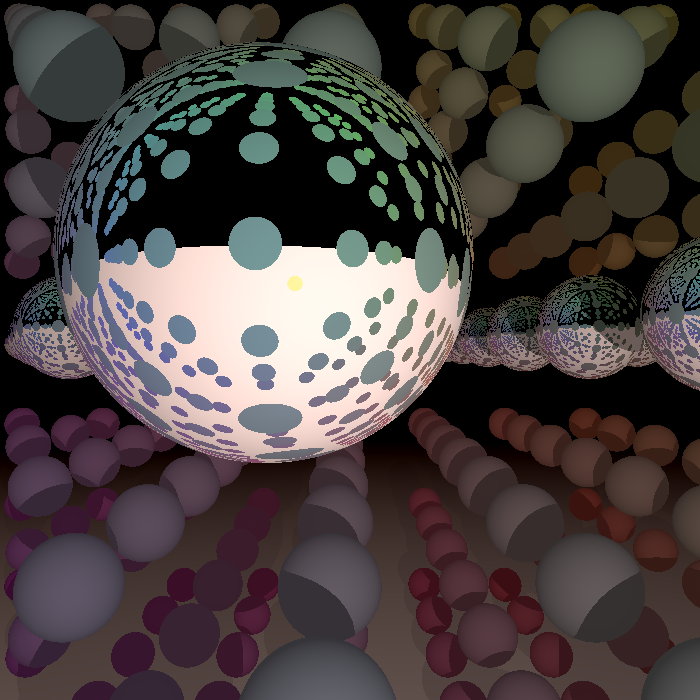
\includegraphics[width=90mm]{reflections.png}
\caption{Reflections that only take into account ambient lighting}
\label{fig:reflections}
\end{figure}

\subsection{User Interface}
The user interface was implemented in GTK+ (see figure \ref{fig:raytracerui}), with the rendered image being displayed in a \texttt{GtkImage}. This is inefficient, as the image is rendered on the GPU, copied to the CPU, copied to the \texttt{GtkImage}, then pushed back to the GPU. An alternative that trades increased complexity for more performance would be taking advantage of OpenCL's OpenGL interoperability features to draw the image.

\begin{figure}[ht!]
\centering
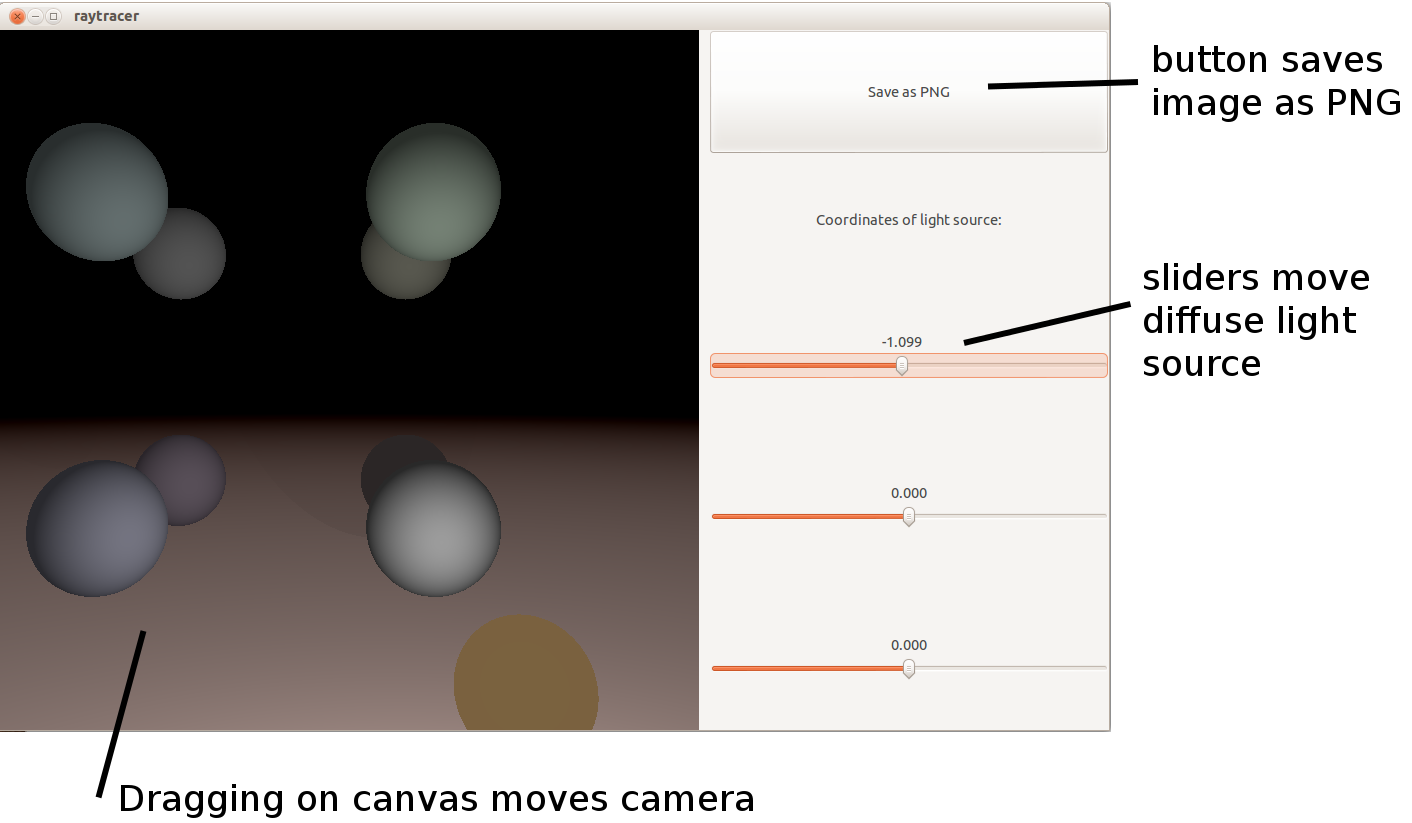
\includegraphics[width=120mm]{raytracer-ui.png}
\caption{Raytracer user interface}
\label{fig:raytracerui}
\end{figure}

\subsection{Performance}
The raytracer is able to render a 700x700 pixel test scene with 1000 spheres and a moveable diffuse light source at speeds that make it interactive (see figure \ref{fig:testscene}). Using the CPU, this scene takes 1.28 seconds per frame (0.78 frames per second). Using the Radeon 7970, the scene takes 0.055 seconds per frame (18 frames per second). If the number of spheres is reduced to 216, the Radeon 7970 can render the scene at 60 frames per second.

\begin{figure}[ht!]
\centering
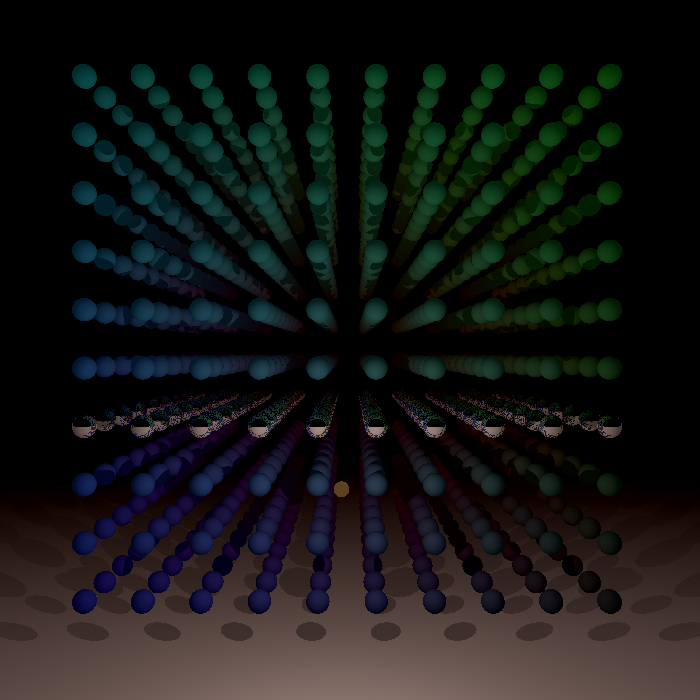
\includegraphics[width=90mm]{scene.png}
\caption{Test scene, featuring 1000 spheres and ground plane}
\label{fig:testscene}
\end{figure}

\subsection{Discarding Frames}
The sliders generate GTK+ events, which are processed in callback functions like \texttt{motion\_notify()}. These callbacks call \texttt{run\_kernel()}, which renders the frame. This blocks the main program thread, but mouse drag events on the image still get queued. The effect is that the program can get more and more behind when rendering frames if events are added faster than frames can be rendered. This makes the raytracer feel unresponsive.

To prevent this from happening, after rendering a frame, the callbacks discard all the events on the GTK+ event queue that could cause a new frame to be rendered. This is done by having an \texttt{in\_handler} flag that is set when a callback that is rendering a frame is running. All callbacks that can render a frame check to see if \texttt{in\_handler} is set, and if so, return without rendering the frame. Immediately after rendering a frame, a callback runs this loop:

\begin{lstlisting}
while ( gtk_events_pending() )
  gtk_main_iteration();
\end{lstlisting}

This causes all the queued GTK+ events to be processed; because the \texttt{in\_handler} flag is set, any other callbacks in the queue do not render a frame. The end result is that all the events that could render a new frame are flushed from the queue.

%%%%%%%%%%%%%%%%%%%%%%%%%%%%%%%%%5
\section{Mankalah Minimax AI}
This part of the project implemented a minimax player for the Mankalah game introduced in CS 212. Minimax is a much harder algorithm to implement on a GPU than a raytracer, because the minimax tree has dependencies between nodes, and the parallelism is less obvious.

\subsection{Strategy}
Following previous work on another minimax player implemented in CUDA\cite{rockisuda10}, the minimax tree is broken up into layers. On the CPU, the first layers of game boards in the minimax tree are computed and the bottom-level leaf nodes of that tree are put into a C++ vector. The boards in the vector are copied over to the GPU, where 4 more levels of minimax are computed. Because the Mankalah minimax tree has a branching factor of 6, the overwhelming majority of the work is done in the bottom 4 levels of the tree (see figure \ref{fig:minimaxdiagram}).

\begin{figure}[ht!]
\centering
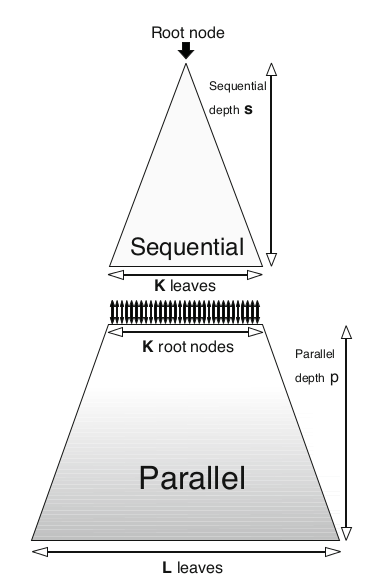
\includegraphics[width=50mm]{minimax-diagram.png}
\caption{Sequential and parallel segements of minimax tree, taken from Rocki and Suda\cite{rockisuda10}.}
\label{fig:minimaxdiagram}
\end{figure}

The algorithm run on the GPU for evaluating the bottom layers of the minimax tree is as follows:

\subsubsection{Generating boards}
In this step, the game boards that represent the game tree for the next number of moves are generated from the start board. The tree is stored in global memory in an array, where the child of the node stored at location n in the array is at location 6n + 1. This can be computed in O(log(n)) time with $n^{d}$ threads, by having the first thread compute the first node, 6 threads compute the first level of child nodes, 36 threads compute the second level, and so on.

\subsubsection{Evaluating boards}
In the standard minimax algorithm, the evaluate function needs to be computed only for boards at the leaf nodes of the game tree. Because all threads execute the same instruction counter, however, it is not slower to run the function on all the generated boards. This saves time in a later step, as should the game end at a stage before the bottom level of the minimax tree, the board is already evaluated.

\subsubsection{Minimax}
The minimax scores at a node can be computed in O(log(n),n) time by using $n^{d-1}$ threads to compute the minimax values for the nodes one level above the leaf nodes, $n^{d-2}$ threads to compute the minimax values for the nodes 2 levels about the leaf nodes, and so on. After this process, the parent node for the game tree stores the minimax value for the tree.

\subsubsection{Limitations}
Because the boards are stored in local memory, and there are sequential dependencies between these steps, all threads for one of these minimax trees must be in the same workgroup. On the Radeon 7970, the maximum work group size is 256. Therefore, for Kalah, with a branching factor of 6, a minimax tree of 4 levels ($6^0 + 6^1 + 6^2 + 6^3 = 259$ nodes) was used, with a workgroup size of $6^3 = 216$. Since there were more nodes in the tree than threads in the workgroup, some threads had to evaluate 2 boards.

\subsection{Increasing Search Depth}
Because of memory bottlenecks, there is a limit to how many GPU minimax instances can be dispatched efficiently. On the test system, 10 levels of sequential minimax was optimal for performance. As well, as Rocki and Suda\cite{rockisuda10} noted, the search tree has to be traversed twice at this level, once to determine what the leaf nodes are, and second to run the minimax reduction on the nodes.

Therefore, to gain more search depth, another level of sequential minimax was run above this first round of sequential minimax. Adding more levels at the topmost level of minimax increased the depth of the search but not the number of GPU instances dispatched at one time. Only one traversal of the search tree is necessary at this step.

\subsection{Performance}
\subsubsection{Optimal Sequential Depth}
One optimization question is for a minimax tree of a given depth how many levels shuld be computed in each of the 3 minimax stages. The GPU portion is fixed at 4 levels, so the distribution needs to be between the two sequential minimax stages. On the test system, the optimal allocation was to do 10 levels on the CPU before moving the boards to the GPU.

\subsubsection{Speedup}
A recursive sequential algorithm was implemented for performance comparisons. As the table below demonstrates, the using the GPU yielded about a 10x speedup once the problem became sufficiently large. A 10x performance increase for a game with a branching factor of 6 means that the player can look another move ahead in the game.

\begin{tabular}{| l | l | l | l | l |}
  \hline
  Depth & Sequential (s) & CPU OpenCL (s) & GPU OpenCL (s) & Speedup\\
  \hline
  4 & 0.000068 & 0.000656 & 0.000919 & 0.07x \\
  5 & 0.000343 & 0.008957 & 0.000907 & 0.37x \\
  6 & 0.001658 & 0.004544 & 0.001054 & 1.57x \\
  7 & 0.008301 & 0.023702 & 0.001382 & 6.00x \\
  8 & 0.040561 & 0.102351 & 0.005487 & 7.39x \\
  9 & 0.203477 & 0.516266 & 0.021644 & 9.40x \\
  10 & 0.980497 & 2.61265 & 0.1048 & 9.35x \\
  11 & 4.80143 & 11.0873 & 0.438745 & 10.9x \\
  12 & 23.4349 & 60.0211 & 2.23596 & 10.5x \\
  13 & 113.512 & 231.792 & 9.41622 & 12.1x \\
  \hline
\end{tabular}
Since minimax is an embarrasingly parallel problem, a parallel CPU implementation should be able to achieve a speed of $\frac{sequential}{\# cores}$. Since the OpenCL parallel implementation was worse on the CPU than the sequential implementation, which itself can be sped up 4 times on the test system, this illustrates how algorithms tuned for GPUs are very different than ones tuned for CPUs.

\subsection{Testing}
Along with testing of each of the GPU minimax algorithm's components, I used fuzz testing to ensure that the output of the GPU minimax algorithm was the same as the output of the sequential CPU minimax implementation. This was done by generating random valid boards then running both algorithms on them and comparing the output.

\subsection{Sharing Code Between Host and Device}
In order to avoid code duplication for the logic for Mankalah boards, the code in \texttt{board.c} and a few other files is used both on the host and device side. To consolidate all a kernel's dependencies into one file, I used the preprocessor to \texttt{\#include} many \texttt{.c} files into one source file. I have tried consistently use the extension \texttt{.cl.in} for OpenCL source files that need to be preprocessed before they will compile.

For data structures passed between the host and device, a shared header file can be used. However, it is important to ensure that the layout of the structures are exactly the same. Notably, fundamental times like an \texttt{int} on the device side is not guaranteed to be the same size as an \texttt{int} on the host side. OpenCL provides types on the host prefaced with \texttt{cl\_} that are guaranteed to be the same size as the type without the prefix on the client side (for an \texttt{int} on the device side, a \texttt{cl\_int} is necessary on the host side). I used preprocessor macros to use the correct types depending on where code is compiled.

\subsection{Tree Structures in OpenCL}
Because there is no dynamic memory allocation in OpenCL, I have stored all trees in arrays. It is common to store binary trees in arrays, where the first child of the node at location $n$ is at location $2n$, and the second at $2n + 1$. This can be generalized to trees of other branching factors. Support functions for this data structure can be found in \texttt{kalah/tree\_array.c}.

%%%%%%%%%%%%%%%%%%%%%%%%%
\section{Economics Simulation}
As a larger, more complex problem, I worked on implementing a GPU version of an economics simulation used for research in Calvin's economics department.\cite{ditta13} The simulation already exists in Python, but it takes on the order of weeks to run. The simulation consists of a number of agents, which each hold a number of resources, that can harvest resources, invent machines to make harvesting resources more efficent, and trade resources and machines with each other.

This problem has promise for a speedup with a GPU's massive parallelism. Each of the agents in the simulation is largely independent, and most of the decisions that agents have to make need to evaluate the relative worth of their resources. Therefore, there is a natural mapping of one hardware thread to one resource, with each agent mapped to its own workgroup.

I did not complete the reimplementation of the simulation, but have met my objective of applying GPU computing to a complex, real-world problem. The Societies paper\cite{ditta13} breaks the simulation into 6 phases, of which the first 3 are non-trivial, the fourth is very complex, and the last 2 are trivial. I implemented the first 2 phases. This was enough to encounter difficult problems that required very different algorithms to efficiently solve on a GPU.

\subsection{Phase 1: Resource Extraction}
In this phase, agents harvest resources while there is time left in the ``day''. In each round, agents choose one of the resources that is most valuable for them to have one more unit of. Agents gain experience extracting resources, which reduces the amount of time needed to extract that resource.

The challenges implementing this phase were implementing the maximum and minimum algorithms, creating a mechanism for threads to create a variable-size array of options, and finding a random number generator.

\subsubsection{Array Maximum and Minimum}
Several times in this simulation, I needed to find the maximum or minimum in an array without modifying the values in the array. The most efficient way to do this with at least 1 thread for every 2 elements is to build a max/min tree, since this allows the maximum or minimum to be found in O(log(n),n) time. Unfortunately, for an array with n elements, this requires a scratch array in \texttt{\_\_local} memory of $\frac{n}{2}$ elements.

The algorithm has two phases. In the first phase, $\frac{n}{2}$ threads compare 2 elements of the original array, and put the largest in the scratch array. In the second phase, $\frac{n}{4}$ threads compare 2 elements of the scratch array, and put the maximum/minimum of the two values in the location of the first value. The second phase iterates, each time with half as many threads, until there is one value left, which is the minimum/maximum.

The implementation of this algorithm is in \texttt{societies/util/max\_min.cl}. This implementation also includes the ability to pass in a mask array, which allows the algorithm to ignore certain values in the array. This permits using the algorithm multiple times to find the maximum/minimum n elements in an array. (See the \texttt{max\_n\_indices()} function.)

\subsubsection{Variable-length Arrays}
There are cases where one thread needs to make a choice between different values on behalf of the workgroup. One implementation of this idiom can be found in \texttt{societies/util/choose\_thread.cl}, where several threads can register their ability to be chosen, then one thread randomly makes a choice between them. Since not all threads want to be chosen, there needs to be a data structure that can hold a variable number of elements and that all threads can add elements too.

This data structure can be implemented in OpenCL with an atomic counter variable in \texttt{\_\_local} memory initialized to 0, with an array in \texttt{\_\_local} memory that is large enough for the maximum possible number of elements. When a thread wants to add an element, it calls the OpenCL-builtin \texttt{atomic\_inc()} function to increment the counter, and puts a value in the array at the position that \texttt{atomic\_inc()} returns, which is the previous value of the counter variable. After all threads have finished adding values to the array, the counter variable holds the number of items in the array.

\subsubsection{Random Numbers}
Many of the Societies algorithms required a source of random numbers. On a GPU, this is difficult because there is no hardware source of random numbers, and PRNGs require a unique seed per workgroup so that each workgroup does not generate the same sequence of random numbers. I made use of the MWC64X random number generator, which is ideal for GPUs because it requires very little state to be preserved across runs. I found an OpenCL implementation which was verified against statistical tests.\cite{mwc64x}

\subsection{Phase 2: Resource Trading}
The agents are able to trade resources in pairs. The algorithms from the previous phase were sufficient for implementing this phase, except that there had to be an efficient way to randomly pair agents while ensuring that each agent was only in one pair. My solution was to generate a random permutation of the numbers $0 \cdots n-1$ using the ``inside-out'' Fisher-Yates shuffle, where $n$ is the number of agents, on the CPU. This permutation is copied to GPU, where one workgroup is assigned to each pair of agents.

\subsection{Testing}
One weakness of the Python Societies code is that it is not written in a way that makes it easy to test. I made sure to make my code very clean  and wrote unit tests for all my functions, so that my code will be useful to the Societies project in the future. The algorithms I developed to find the maximum and minimum elements in an array I was also careful to test; this code should be useful as a reference for others doing similar work in OpenCL.

\subsection{Kernel Size}
The OpenCL kernels for Societies were relatively large. This is because \texttt{\_\_local} memory cannot be preserved across kernel runs, so splitting up complex tasks into several kernels was not feasible. The Mankalah player has 3 stages that are independent except that the values in \texttt{\_\_local} memory needed to be kept. This is a limitation of the hardware that leaks through as complexity for programmers.

My strategy was to test each of the segments of the kernels independently, so that it was still possible to debug one section of code at a time. However, certain kinds of bugs like race conditions due to missing barriers can only be tested with the kernel as a whole.\footnote{As an aside, CPUs are much more vulnerable to synchronization errors than GPUs, because on a GPU, all hardware threads in a workgroup share an instruction pointer. In fact, the AMD OpenCL backend removes barriers that are made unnecessary by the GPU's architecture.}

\subsection{Configuration Values}
There were several configuration values that are known at kernel compile time, but at host run time. Some of them, like the number of agents in the simulation, needed to be accessible as preprocessor macros. Another advantage of passing configuration values from the host to the device using preprocessor macros rather than inside a configuration object is that memory accesses can be cut out of 

\subsection{Partial Completion}
As I was starting work on the third phase of the simulation, it was getting unwieldly to program the large and complex kernels. I found that managing buffers of \texttt{\_\_local} memory were the largest source of complexity, and thought approaching that problem would be ultimately more fruitful than finishing the increasingly complex parts of the Societies simulation. In particular, the method by which agents traded higher-order devices in the simulation was complicated, only partially documented in the Societies paper, and the Python source code was obtuse. It would have been more of an exercise in implementing specifications than computer science research.

%%%%%%%%%%%%%%%%%%%%%%%%%%%%%%%%%%%%%%%%%%
\section{\_\_local Memory malloc()}
One problem I ran across when implementing the Societies code was that most functions required many parameters to pass around scratch \texttt{\_\_local} memory that was needed by some algorithm several function calls deep. These scratch buffers needed to be declared at the beginning of a kernel rather then when they were actually used, and I had to keep track of exactly how large they needed to be. Also, because \texttt{\_\_local} memory usage restricts the number of hardware threads that can be concurrently running on the GPU, it is important to minimize the amount used, which means reusing the same buffers when possible. The result is that the complexity of managing buffers of \texttt{\_\_local} memory became a bottleneck.

Because the sizes of all these buffers is known at compile-time, and OpenCL does not support recursion or function pointers, simple static analysis is enough to determine the maximum amount of \texttt{\_\_local} memory a kernel needs. This should make it easy to shift the accounting burden from the programmer onto a tool.

As well, OpenCL does not support global variables, so any state used by a \texttt{malloc()}-like tool needs to be passed as a parameter to every function. This is inconvenient for the programmer, and should be easy for a tool to write into a program.

\subsection{Integration with Clang}
The Clang C-family compiler is written to be extensible. Clang's abstract syntax tree (AST) includes references to the text that every AST node is built from, which is meant to make it easy for tools to analyze and rewrite source code. Clang's \texttt{Rewriter} class allows for sections of source code to be added, deleted, and moved around. Clang also is used in many OpenCL vendors' backends, which means it natively supports the OpenCL keywords like \texttt{\_\_kernel} and adds these annotations to its AST.

Therefore, this tool links against Clang, and creates an instance of an OpenCL compiler that does semantic analysis but stops before code generation. By using Clang's AST nodes and its \texttt{Rewriter} class, this tool offloads the heavy lifting of parsing and rewriting C source code to Clang.

Because of the tight integration with Clang, the tool is vulnerable to modifications to Clang's internals. The tool was developed against Clang 3.2 and LLVM 3.2.

\subsection{Phase 1: Computing Maximum Allocation}
The tool registers hooks into Clang's AST processing methods. Whenever a function declaration is encountered, the tool generates a new node in a call graph. Then, whenever a function call or a call to \texttt{local\_malloc()} or \texttt{local\_free()} is encountered, the tool adds these actions to the node in the call graph. Clang's AST nodes for the \texttt{local\_malloc()} and \texttt{local\_free()} have methods that make it easy to get a numerical value for the amount of memory allocated or freed, even when that value is an expression or defined by a preprocessor macro.

After all nodes in the AST have been visited, this call graph is guaranteed to have no cycles, because OpenCL does not support recursion. Therefore, in this call tree, the maximum amount of memory allocated by a function is the maximum amount allocated by any of a function's children plus any memory the function has allocated at the same time.

\subsection{Phase 2: Program Rewriting}
The tool then revisits all the nodes in the AST again, and rewrites function declarations and calls. To the kernel function, it inserts initialization code and allocates the \texttt{\_\_local} memory buffer at the size computed in the previous phase. The tool adds a state object to every function call and declaration, so that that state object is accessible anywhere in the program.

\subsection{Including Runtime Code}
The actual code for the \texttt{local\_malloc()} and \texttt{local\_free()} functions needs to be bundled with the rewritten code. One difficulty is that these functions have a different signature before and after rewriting (because the state object is added as a parameter). Also, OpenCL does not support including header files in its compiler. Therefore, the rewriter injects the needed run-time code at the beginning of the program, with the signatures of \texttt{local\_malloc()} and \texttt{local\_free()} as the programmer expects them defined as prototypes. These prototypes are visible only when a preprocessor macro is defined. This allows Clang to parse the code without errors. This code is left in after rewriting, but the preprocessor macro is no longer defined. This exposes the run-time signatures of \texttt{local\_malloc()} and \texttt{local\_free()} along with their code.

I wrote a small tool that allowed me to embed this source code into the executable of the tool, which means that the tool does not need to find that source code file to be able to be used.

\subsection{Results}
An example program using \texttt{local\_malloc()} is in \texttt{local\_malloc/example}. This example uses the rewriting tool tool to rewrite a kernel using \texttt{local\_malloc()}, then runs it using the OpenCL framework. This program only needed 9 lines devoted to rewriting the kernel and running it on an OpenCL device.

%%%%%%%%%%%%%%%%%%%%%%%%%%%%%%%%%%%%%%%%%%
\section{Conclusions}
OpenCL was difficult to work with, and the limitations it imposed made it difficult to do otherwise-simple tasks like find minimum values in an array. There is a long way to go before GPUs are accessible to non-specialist developers with OpenCL. OpenACC, which is built into a C/C++ compiler and uses \texttt{\#pragma} similar to OpenMP is a promising route. However, I do not think OpenACC would have reduced the complexity of writing larger applications like the Societies simulation. The framework was successful at making OpenCL easier to use on the host side, but the OpenCL language created complexity on the device side. More device-side language features, like \texttt{local\_malloc()} would better serve to make the GPU easier to use than more host-side improvements.

The Mankalah player and Societies simulation were excellent exercises at designing data-parallel algorithms to solve problems that are not obviously data-parallel. Because of the performance and power benefits of data-parallel architectures, the kind of thinking needed to design these algorithms will only become more relevant. The Mankalah player was also a useful exercise at designing an application that made use of the strengths of all the parts of a heterogeneous architecture. 

%%%%%%%%%%%%%%%%%%%%%%%%%%%%%%%%%%%%%%%%%%%
\section{Future Work}
Some kind of standard library for OpenCL kernels that could perform tasks like sorting arrays in \texttt{\_\_local} memory efficiently, generating pseudorandom numbers, or finding the minimum $n$ values in an array would make complex kernels much easier to write. In general, OpenCL's API encourages writing small kernels that do one thing, but this conflicts with GPU architecture where it is faster to keep data in \texttt{\_\_local} memory while a large kernel does a lot of processing work on it.

There is a lot of space for programming languages to reduce the complexity of writing kernels. The \texttt{local\_malloc()} tool is an example, but the abstractions are able to go higher. OpenCL requires programming from the vantage point of an individual hardware thread, but the individual threads are usually coordinated into tasks, like finding the minimum in an array. Having separate languages or layers of abstraction for the thread-level versus task-level views of a kernel would be useful.

\bibliographystyle{plain}
\bibliography{final-report}

\end{document}
